% Options for packages loaded elsewhere
\PassOptionsToPackage{unicode}{hyperref}
\PassOptionsToPackage{hyphens}{url}
%
\documentclass[
]{article}
\usepackage{amsmath,amssymb}
\usepackage{lmodern}
\usepackage{iftex}
\usepackage{graphicx}
\ifPDFTeX
  \usepackage[T1]{fontenc}
  \usepackage[utf8]{inputenc}
  \usepackage{textcomp} % provide euro and other symbols
\else % if luatex or xetex
  \usepackage{unicode-math}
  \defaultfontfeatures{Scale=MatchLowercase}
  \defaultfontfeatures[\rmfamily]{Ligatures=TeX,Scale=1}
\fi
% Use upquote if available, for straight quotes in verbatim environments
\IfFileExists{upquote.sty}{\usepackage{upquote}}{}
\IfFileExists{microtype.sty}{% use microtype if available
  \usepackage[]{microtype}
  \UseMicrotypeSet[protrusion]{basicmath} % disable protrusion for tt fonts
}{}
\makeatletter
\@ifundefined{KOMAClassName}{% if non-KOMA class
  \IfFileExists{parskip.sty}{%
    \usepackage{parskip}
  }{% else
    \setlength{\parindent}{0pt}
    \setlength{\parskip}{6pt plus 2pt minus 1pt}}
}{% if KOMA class
  \KOMAoptions{parskip=half}}
\makeatother
\usepackage{xcolor}
\IfFileExists{xurl.sty}{\usepackage{xurl}}{} % add URL line breaks if available
\IfFileExists{bookmark.sty}{\usepackage{bookmark}}{\usepackage{hyperref}}
\hypersetup{
  hidelinks,
  pdfcreator={LaTeX via pandoc}}
\urlstyle{same} % disable monospaced font for URLs
\setlength{\emergencystretch}{3em} % prevent overfull lines
\providecommand{\tightlist}{%
  \setlength{\itemsep}{0pt}\setlength{\parskip}{0pt}}
% \setcounter{secnumdepth}{-\maxdimen} % remove section numbering
\ifLuaTeX
  \usepackage{selnolig}  % disable illegal ligatures
\fi

\title{Corruption is not enough}
\author{Butter}
\date{December 2022}

\begin{document}
\maketitle
\setcounter{tocdepth}{2}
\tableofcontents

\hypertarget{butter}{%
\section{Butter}\label{butter}}

Butter is a DAO governance system. Its objective is to align DAO
governance outcomes to DAO objectives through the direct application of
incentives.

This paper describes a prototype, Molten, that attempts to influence DAO
stakeholders and governance participants to cooperate using one-off
payments.

\hypertarget{summary}{%
\section{Summary}\label{summary}}

One token, one vote mechanisms are the most popular governance
mechanisms used by DAOs. However, one token, one vote and other token
voting systems are plutocracies and widely considered vulnerable to
\href{./problems.md\#corruption-problems}{corruption} and
\href{./problems.md\#attack-problems}{attack}.

Large or mature DAOs, and many newer DAOs, have introduced vote
delegation in an attempt to scale governance and alleviate the risks of
plutocracy.

However, many recent and well-known examples of plutocracy involve DAOs,
including ENS DAO, Sushi DAO, and MakerDAO, in which vote delegation is
allowed and often enforced.

We examine the DAO governance problem space and highlight promising
in-market solutions, including hybrid governance, metagovernance, and
market-based governance.

We propose cryptoeconomics, a system of economic incentives designed to
produce behaviours at the micro scale that create desirable, emergent
properties at the macro scale, as a viable solution space for further
exploration.

Finally we describe Molten, a system that aims to address the risks
related to plutocracy in DAO Governance using incentives designed to
make corruption an unprofitable strategy.
\hypertarget{motivation}{%
\section{Motivation}\label{motivation}}

\hypertarget{decentralised-autonomous-organisations}{%
\subsection{Decentralised Autonomous
Organisations}\label{decentralised-autonomous-organisations}}

DAOs are a novel form of organisation, uniquely enabled by blockchains.

The components of an organisation include, but are not limited to:

\begin{enumerate}
\def\labelenumi{\arabic{enumi}.}
\tightlist
\item
  an \textbf{objective} or \textbf{purpose}
\item
  a \textbf{membership policy} that produces a set of members,
  e.g.~holds shares, holds tokens, is contracted, etc.
\item
  an~\textbf{allocation mechanism}~which defines how the organisation
  allocates resources
\item
  a~\textbf{standardised store of value} which defines how the
  organisation values and represents its resources, e.g., currency,
  equity, tokens
\item
  a~\textbf{governance mechanism}~which defines how to update the
  organisation's properties, e.g.~membership policy, allocation
  mechanism, etc.
\end{enumerate}

DAOs, through their use of blockchains, claim to provide the benefits of
large-scale coordination without the downsides of centralization. These
downsides inlcude capture, corruption, and collusion----problems that
undermine our most-trusted institutions.

Generally, DAO proponents expect DAOs to replace traditional
institutions in the provision of public, common, or club goods. When
these institutions fail, centralisaion is usually a root cause,
e.g.~bureaucracy, corruption, principal-agent problems.

In practice, however, it appears that DAOs do not offer effective
solutions to these problems and often move them elsewhere in the value
chain\href{https://kelsienabben.substack.com/p/towards-a-model-of-resilience-in}{1}.
Current DAO implementations, therefore, remain vulnerable to the same
issues faced by our incumbent institutions.

\hypertarget{dao-governance}{%
\subsection{DAO Governance}\label{dao-governance}}

\emph{DAO governance involves a network of participants that coordinate
to make decisions, \textbf{without a centralised actor with privileged
rights,} in pursuit of some goal or outcome, and is formalised or
defined under set of shared context(s), e.g.~a geography, the law, a
market, a cause, etc.}

DAOs, like other organizations, implement internal policies that govern
their components and the interactions between them. This includes the
law in the case of nations, compensation, taxation, resource allocation,
social choice, etc.

DAOs are similarly governed by external policies enforced by their
environment, such as the law in the case of corporations, market forces,
international relations, physics, blockchain protocols, etc.

Governance mechanisms can, therefore, be considered the component of
DAOs responsible for mediating all DAO components. They are, in turn,
mediated by their environment and competing DAOs.

For the purposes of improving its outcomes, a DAO's governance mechanism
could be considered the DAO itself. Therefore, we expect improvements in
DAO Governance to be an effective means to realising the expected
positive value of DAOs on society.

\hypertarget{dao-governance-models}{%
\subsection{DAO Governance Models}\label{dao-governance-models}}

\emph{Note: We recognise that token-voting, though democratic in nature,
is far from a democracy in the literal sense. However, we will use the
term democracy to adhere to market convention}

Models include:

\begin{itemize}
\tightlist
\item
  Direct Democracy
\item
  Representative Democracy
\item
  Reputation-based Voting
\end{itemize}

\hypertarget{direct-democracy}{%
\subsubsection{Direct Democracy}\label{direct-democracy}}

\textbf{\emph{One token, one vote on every proposal}}

\textbf{Description}

In a direct democracy, token-holders make decisions by voting on
proposals, where each token is equivalent to a vote. Currently, this is
the governance mechanism used by the majority of DAOs, especially
smaller, younger DAOs.

Governance must configure the following parameters:

\begin{itemize}
\tightlist
\item
  Who has the right to create a proposal
\item
  How to convert token votes to a decision, e.g.~majority-rule,
  supermajority, quorum rules
\end{itemize}

\textbf{Benefits}

\begin{itemize}
\tightlist
\item
  Bundling financial upside and governance rights aligns risk and
  responsibility, which incentivises those with the most to gain from
  price appreciation to make decisions that directly or indirectly
  maximise price appreciation
\item
  This replicates features of the equity system, which makes it simple
  for holders to understand
\end{itemize}

\textbf{Limitations}

\begin{itemize}
\tightlist
\item
  Keeps out those who may be affected by governance but don't have the
  capital to acquire governance rights
\item
  Tends towards plutocracy which, if left unchecked, leads to failure
  through a focus on price appreciation, regardless of negative
  externalities
\end{itemize}

\textbf{Examples}

\begin{itemize}
\tightlist
\item
  PleasrDAO, Aavegotchi, VitaDAO
\end{itemize}

\hypertarget{representative-democracy}{%
\subsubsection{Representative
Democracy}\label{representative-democracy}}

\textbf{\emph{One token, one vote on every proposal with vote
delegation}}

\textbf{Description}

In a representative democracy, token-holders make decisions by voting on
proposals, where each token is equivalent to a vote, but can also
delegate their voting power to a representative. Delegated voting is
increasingly becoming the most popular governance mechanism, especially
for mature, large DAOs.

Governance must configure the following parameters:

\begin{itemize}
\tightlist
\item
  Who has the right to create a proposal
\item
  How to convert token votes to a decision, e.g.~majority-rule,
  supermajority, quorum rules
\item
  Which rights can be delegated and to whom
\end{itemize}

\textbf{Benefits}

\begin{itemize}
\tightlist
\item
  Aligns incentives by unbundling financial risk and governance power
  and allocating them to domain experts
\item
  Allows governance rights to accrue to representatives~whom voters
  believe are best placed to represent their preferences
\item
  Reduces voter apathy
\end{itemize}

\textbf{Limitations}

\begin{itemize}
\tightlist
\item
  As delegation scales, the nuance of voter preferences is diluted to
  the preferences of a smaller subset of voters, i.e.~the delegates,
  which is less representative of the population
\item
  Forces the voter to find a single delegate who represents their entire
  range of preferences across all possible decisions (though tokens
  could be split across wallets or delegation functionality enhanced)
\item
  Allowing voters to delegate enables a more persistent form of voter
  apathy, as seen in our traditional political system
\end{itemize}

\textbf{Examples}

\begin{itemize}
\tightlist
\item
  Uniswap, Gitcoin, Compound, ENS, MakerDAO, AAVE, Radicle, Nouns DAO
\end{itemize}

\hypertarget{reputation-based-voting}{%
\subsubsection{Reputation-based Voting}\label{reputation-based-voting}}

\textbf{\emph{One person, one vote OR One contribution/reputation unit,
one vote on every proposal}}

\textbf{Description}

Non-transferable voting based on your membership, reputation and, or
contribution.

\textbf{Benefits}

\begin{itemize}
\tightlist
\item
  more equitable relative to token-weighted voting, i.e.~meritocratic
\item
  aligns contribution and power
\item
  does not produce plutocracy
\end{itemize}

\textbf{Limitations}

\begin{itemize}
\tightlist
\item
  only as performant as the system's ability to measure contributions
  and assign relative value
\item
  assumes equal exposure to externalities
\item
  inability to express preference intensity
\end{itemize}

\textbf{Examples}

\begin{itemize}
\tightlist
\item
  Optimism's Citizen's House
\end{itemize}
\hypertarget{problems}{%
\section{Problems}\label{problems}}

\hypertarget{problem-space}{%
\subsection{Problem Space}\label{problem-space}}

The problem space is defined as DAO Governance, in particular:

\begin{itemize}
\tightlist
\item
  DAO Governance Corruption, including Capture, Collusion, and
  Opportunism
\item
  DAO Governance Attacks, including Capital Structure Exploitation
\end{itemize}

\hypertarget{properties}{%
\subsection{Properties}\label{properties}}

\begin{itemize}
\tightlist
\item
  \textbf{Stakeholder.} Any individual, collective, or entity that
  experiences externalities due to the actions of the DAO,
  e.g.~Token-holder, user, delegate, staker/miner, etc.
\item
  \textbf{Participant.} Any individual, collective, or entity that
  participates in governance
\item
  \textbf{Preference.} A stakeholder's subjective, comparative
  evaluations over a range of options, e.g.~a miner prefers to increase
  the block reward, over reducing rewards or keeping rewards constant
\item
  \textbf{Objectives.} The goal or set of goals that constitute the
  DAO's organizing purpose, e.g.~``Buy the constitution'', ``Fund Public
  Goods''
\item
  \textbf{Acts.} The set of actions or decisions the DAO's governance
  mechanism is able to produce and its stakeholders consider, e.g.~Add a
  new asset as collateral in our lending protocol, remove a particular
  voter's voting power, increase token supply, offboard a contributor,
  suspend the protocol
\item
  \textbf{Outcomes.} The set of outcomes the DAO's governance mechanism
  is able to achieve through its actions, e.g.~Token Price increases or
  remains stable, protocol users increase
\end{itemize}

\hypertarget{dimensions}{%
\subsection{Dimensions}\label{dimensions}}

To measure the effectiveness of a DAO's governance, we consider the
following dimensions:

\begin{itemize}
\tightlist
\item
  \textbf{Stakeholder Representation.} The distribution of voting power
  relative to DAO stakeholders, i.e.~users, token holders, stakers,
  liquidity providers, etc.
\item
  \textbf{Preference Representation.} The degree to which governance
  participants are able to express their preferences with respect to the
  DAO's objectives, e.g.~I do not believe the voting mechanism is
  legitimate
\item
  \textbf{Alignment.} The consistency of a decision when compared to a
  desired outcome
\item
  \textbf{Coherence.} The consistency of a series of decisions when
  compared to one another, with respect to a desired outcome
\item
  \textbf{Legitimacy.} Power granted by governance participants to the
  governance mechanism through their ongoing implicit agreement to be
  bound by its decisions
\end{itemize}

\hypertarget{problems-1}{%
\subsection{Problems}\label{problems-1}}

\hypertarget{corruption-problems}{%
\subsubsection{Corruption Problems}\label{corruption-problems}}

\hypertarget{opportunism}{%
\paragraph{Opportunism}\label{opportunism}}

Where a single stakeholder or group of stakeholders is rewarded for
acting in their own self interest while punishing all other stakeholders
and producing outcomes that do not align with the DAO's objectives.

\textbf{Example:} Proposing or voting for salary increases or against
salary cuts during a budget-cutting exercise.

\textbf{Symptoms:} - Deviation between outcomes and objectives -
Increase in actions or decisions that do not align with objectives -
Illegitimate diversion of funds

\hypertarget{capture}{%
\paragraph{Capture}\label{capture}}

Where a minority group of stakeholders possess the power to dictate the
DAO's actions to serve their own preferences while punishing all other
stakeholders and producing outcomes that do not align with the DAO's
objectives.

\textbf{Example:} Plutocracy, Bureaucracy

\textbf{Symptoms:} - Deviation between outcomes and objectives -
Increase in actions or decisions that do not align with objectives -
Illegitimate diversion of funds

\hypertarget{collusion}{%
\paragraph{Collusion}\label{collusion}}

Where two or more stakeholders or stakeholder groups that operate within
or outside the boundaries of the DAO cooperate for their mutual benefit,
to the detriment of all other stakeholders and the DAO's ability to
achieve its objectives.

\textbf{Example:}
\href{https://hackingdistributed.com/2018/07/02/on-chain-vote-buying/}{Vote
Buying}

\textbf{Symptoms:} - Deviation between outcomes and objectives -
Increase in actions or decisions that do not align with objectives -
Illegitimate diversion of funds

\hypertarget{attack-problems}{%
\subsubsection{Attack Problems}\label{attack-problems}}

\hypertarget{capital-structure-exploitation}{%
\paragraph{Capital Structure
Exploitation}\label{capital-structure-exploitation}}

Where an individual or group is able to exploit vulnerabilities in the
DAO's governance mechanism to extract capital.

\textbf{Example:} Treasury Drain Attacks, Price Manipulation Attacks,
Arbitrageurs, etc.

\textbf{Symptom:} - Illegitimate diversion of funds
\hypertarget{governance-innovations}{%
\section{Governance Innovations}\label{governance-innovations}}

DAO Governance, unlike corporate and public governance, is both public
and open source. The principles of the open source community, that
anyone can copy and reuse for free, provides many opportunities for
governance innovation----some of which we've shared below.

\emph{Metagovernance,} \emph{Hybrid Governance,} and \emph{Market
Governance} are three categories of governance innovation that may offer
effective solutions with respect to our problem space.

\hypertarget{metagovernance}{%
\subsection{Metagovernance}\label{metagovernance}}

Metagovernance, in the context of DAOs, is the term commonly used to
describe any activity where one governance mechanism, typically a
protocol or a DAO, exerts influence on the governance of another DAO.

Metagovernance is a transparent, often automated, vote-buying mechanism
that incentivizes a target DAO's token-holders to take an action that
benefits the mechanism's stakeholders, e.g.~influence over governance
decisions, direction of token emissions, etc.

Metagovernance creates a secondary set of incentives, or
meta-incentives, that augment the behaviour of the target DAO's
stakeholders.

In one-off instances of metagovernance, such as in the case of Fei and
Index Coop, the Fei team were able to gain influence in AAVE's
governance using Index Coop's AAVE holdings.

There are also extended forms of metagovernance with DAOs whose entire
purpose is to control the governance of other DAOs, such as Convex
Finance.

\hypertarget{curve-emissions-with-convex-finance}{%
\subsubsection{Curve emissions with Convex
Finance}\label{curve-emissions-with-convex-finance}}

Convex was designed to maximise control over CRV emissions on the Curve
protocol.

Convex works by reimplementing Curve's vote-escrow token mechanic to pay
CRV holders with CVX emissions in exchange for locking their CRV tokens
in Convex's contract.

Convex, in turn, locks these CRV tokens using Curve's contracts to
maximize their CRV emissions, which they share with CVX holders, and
voting power, which they use to vote for increased token emissions for
pools selected by CVX holders.

As of this writing, the Convex protocol controls 51\% of all
vote-escrowed CRV, an indicator of the effectiveness of meta-incentives
in one-token, one-vote governance mechanisms.

\hypertarget{redacted-cartel-hidden-hand}{%
\subsubsection{Redacted Cartel, Hidden
Hand}\label{redacted-cartel-hidden-hand}}

Hidden Hand from Redacted Cartel facilitates vote-buying campaigns for
participating DAOs.

Vote buyers, or bribers, can deposit bribes for governance proposals at
participating DAOs and users can delegate governance tokens to the
Hidden Hand protocol. The protocol then distributes votes to maximise
returns for its users in exchange for a 4\% commission of bribes
received.

As an example, as of September 7, 2022, \$851,364~worth of bribes were
deposited for~61~proposals on Aura Finance and \$2,346,024 was deposited
for~27~proposals on Balancer.

Hidden Hand also allows partners to implement their own bribe
marketplaces so users can sell votes to bribers directly.

\hypertarget{fei-asset-listing-on-aave-with-index-coop}{%
\subsubsection{FEI Asset Listing on AAVE with Index
Coop}\label{fei-asset-listing-on-aave-with-index-coop}}

Index Coop, a provider of token indexes, actively encouraged
metagovernance for a small number of the tokens held in their DeFi Pulse
Index, namely Maker, AAVE, and Compound--a service they promoted as
metagovernance-as-a-service.

Under this arrangement, holders of INDEX tokens could use governance
tokens held as part of the index service to make or vote on proposals
within MakerDAO, AAVE, and Compound.

In September 2021, Fei protocol, a stablecoin issuer, created a proposal
to list the FEI token on AAVE, using the AAVE token holdings in Index
Coop's DPI.

AAVE's governance, specifically, requires 80,000 AAVE tokens before a
holder can make a governance proposal. At that time, AAVE was trading at
\$327.04, setting the cost of proposal creation on AAVE at over \$26m.

As a result of metagovernance, the Fei team were able to use \$4m of
INDEX tokens to control over 118,000 AAVE, worth \textasciitilde\$36m,
allowing the team to successfully list their token on AAVE.

\hypertarget{hybrid-governance}{%
\subsection{Hybrid Governance}\label{hybrid-governance}}

Hybrid governance is here defined as the combination of two or more
governance models within a single DAO governance mechanism.

This approach is typically pursued where DAO governance designers
believe that outcomes can be better-aligned to the DAO's objectives by
limiting the influence of stakeholders whose preferences are
over-represented in a one-token, one-vote model.

Hybrid governance can also be implemented to give greater weight to the
preferences of a group of stakeholders who are underrepresented or have
no means to express their preferences except to ``vote with their
feet'', which is a loss for all stakeholders.

Hybrid governance modulates the influence of one set of stakeholders by
distributing voting rights to another set of stakeholders, especially
groups who may be marginalised by the preferences of dominant voters.

Voting power is redistributed until each group is able to provide
sufficient checks and balance on the power of other groups.

\hypertarget{lidos-steth-dual-governance}{%
\subsubsection{Lido's stETH Dual
Governance}\label{lidos-steth-dual-governance}}

LidoDAO's is governed by LDO holders. Unfortunately, users that stake
ETH in the Lido contract receive stETH, which confers the holder no
voting rights.

This structure allows Lido holders to make decisions that benefit LDO
holders at the expense of stETH holders.

The goal of Lido's Dual Governance proposal ``is to prevent the Lido DAO
governance from changing the covenant between the protocol and stakers
without consent from the latter.''

The proposal grants stETH holders a vetocracy over proposals that are
deemed to break the agreement under which users stake their ETH on Lido.
stETH holders can signal their disagreement with a proposal by staking
stETH in a vote escrow contract and once a minimum threshold is reached
the proposal will be temporarily blocked to allow the community to
negotiate. stETH holders can vote to block, amend, or pass the proposal
after negotiations.

This power gives stETH enough power to limit opportunism by LDO token
holders without burdening stakers with ongoing governance overhead.

\hypertarget{optimisms-hybrid-governance}{%
\subsubsection{Optimism's Hybrid
Governance}\label{optimisms-hybrid-governance}}

Optimism, through the Optimism Collective have implemented a bicameral
legislative process, comprising a `Token House' within which voting
powers are granted through token ownership, and a `Citizens' House',
within which voting powers are granted through non-transferrable NFTs or
``soulbound tokens''.

The Citizen's House's remit appears to be reserved for retroactive
public goods funding whereas the Token House has a more traditional DAO
governance remit, e.g.~governance fund~grants, protocol upgrades,
director removal, etc. The team explains that this approach is ``a
large-scale experiment
in~\href{https://vitalik.ca/general/2021/08/16/voting3.html}{non-plutocratic
governance}'' but, so far, there are limited details.

\hypertarget{market-governance}{%
\subsection{Market Governance}\label{market-governance}}

Market Governance is co-opted from
\href{https://en.wikipedia.org/wiki/Market_governance_mechanism}{Market
Governance Mechanisms} to describe a mechanism that leverages the
competitive forces of the open market to influence the behaviour of
stakeholders.

As DAOs have scaled in scope, market cap, and contributors, token-based
governance has created opportunities for corruption and in-fighting,
especially where the DAO's operations are complex.

As the range and diversity of stakeholders increases, and the potential
set of actions and decisions expand, governance must increase its
throughput to accommodate, without creating a self-serving bureaucracy.

\hypertarget{makerdaos-metadaos}{%
\subsubsection{MakerDAO's MetaDAOs}\label{makerdaos-metadaos}}

The solution proposed by Rune in Endgame constitutes a decomposition of
MakerDAO into a single core DAO housing the main functions of the Maker
protocol and a collection of smaller ``MetaDAO'' governance units with
their own governance and governance token. ``MetaDAOs'' have the freedom
to pursue any viable market opportunity, while leveraging the resources
of the core DAO.

This innovation affords MakerDAO the ability to maintain a small number
of governance-controlled parameters for the core protocol, while the
market provides the incentives to steer MetaDAO governance to the
pursuit of new market opportunities.

This governance upgrade is in the process of being deployed at MakerDAO
so its effects are yet to be measured.
\hypertarget{proposal}{%
\section{Proposal}\label{proposal}}

Each governance innovation provides a tool for addressing problems in
DAO Governance.

\emph{Metagovernance} provides a system of secondary incentives to
reward governance participants for taking a set of desired actions,
which is useful for limiting opportunistic behaviour.

\emph{Hybrid Governance} redistributes voting power among stakeholders
using a secondary governance mechanism. The second mechanism provides a
system of checks and balances between the two groups, guaranteeing a
system can never be captured by a single group of voters operating under
a single mechanism.

\emph{Market Governance} decomposes governance into self-contained
organisations, allowing market forces to govern each organization's
decisions. As a result, organizations that become bureaucracies, or
engage in corrupt practices are outcompeted by those that are
consistently productive.

These mechanisms improve stakeholder cooperation and alignment using
three types of incentives. \emph{Metagovernance} incentives are provided
by a mechanism or protocol. \emph{Hybrid Governance} relies on
incentives which are provided by other stakeholders or peers.
\emph{Market Governance} incentives are provided by the market through
competition.

Should governance attack, corruption, or capture be detectable by a
governance mechanism, other stakeholders, or competing mechanisms,
incentives offer an opportunity to offset the proceeds of these acts,
rendering them unprofitable.

Through our investigations in the field of cryptoeconomics, we aim to
design a mechanism or collection of mechanisms capable of providing
sufficient guarantees about cooperative behaviour in DAOs.

Next, we present an initial exploration of the solution space.
\hypertarget{molten}{%
\section{Molten}\label{molten}}

\emph{Molten is WIP. This document will be updated as we conduct ongoing
research and development.}

Molten incentivizes voters to pool their votes to deter opportunistic
behaviour by large token holders.

\hypertarget{actors}{%
\subsection{Actors}\label{actors}}

Molten is designed to coordinate the actions of three actors:

\textbf{Representative.} Stakeholder that wants to accrue voting power
but lacks resources. Equivalent to a delegate in a DAO with vote
delegation.

\textbf{Voter.} Stakeholder that wants protection against large voters
and has adequate resources.

\textbf{Target DAO.} DAO that wants to allocate resources in pursuit of
its objective.

\hypertarget{components}{%
\subsection{Components}\label{components}}

Molten is comprised of:

\textbf{Campaigns.} A period of time within which Voters pool their
tokens in order to delegate voting power to a Representative. Can be
launched by Representative once Campaign threshold is achieved,
e.g.~100,000 governance tokens deposited.

\textbf{Campaign Manager.} Contract that manages all Campaigns,
including types, parameters, and rewards.

\textbf{Molten Pot.} Contract created by Representatives to lock tokens
during a Campaign. Voters deposit and claim tokens from Pots. Deposits
are frozen once a Campaign is launched.

\textbf{Molten Pot Factory.} Contract used to create Pots.

\textbf{Reward.} Fixed token reward, e.g.~30,000 DAI, claimable in
proportion to Voters' Pot claim at the end of a Campaign.

\textbf{mTokens.} Tokens issued to Voters during a Campaign. Each token
represents a proportional claim on the underlying governance tokens and
rewards locked in the Pot contract.

\hypertarget{operation}{%
\subsection{Operation}\label{operation}}

\begin{enumerate}
\def\labelenumi{\arabic{enumi}.}
\item
  Molten uses the Campaign Manager to create a new Campaign Type and
  sets Campaign duration, Target DAO Governance Token (ERC20)
\item
  Representatives create Campaigns and broadcast their Campaign and
  Molten Pot contract address to Voters
\item
  Voters deposit tokens into Molten Pots attached to Representatives
  they believe will pool the most voting power for a Campaign
\item
  Target DAO deposits Reward in the Campaign Manager for the respective
  Campaign Type and sets Campaign threshold
\item
  Once a Molten Pot attached to a Representative exceeds the Campaign
  threshold, the Representative can launch the Campaign. This ends all
  other Campaigns of the same type, allowing Voters to claim tokens from
  the Molten Pots
\item
  Once the Campaign is launched, Molten Pots delegate pooled governance
  token voting power to Representatives, e.g.~AAVE, and issue mTokens to
  Voters, e.g.~mAAVE
\item
  Once the Campaign duration is reached, the underlying governance
  tokens and Rewards are claimable from the Molten Pot \& Campaign
  Manager
\item
  During the campaign, should mToken holders decide that a
  Representative is no longer protecting their interests they can vote
  to terminate the Campaign, removing the Representative's voting power
  and forfeiting the Reward for all parties
\end{enumerate}

\hypertarget{outcome}{%
\subsection{Outcome}\label{outcome}}

Molten combines peer incentives, used to incentivize Representatives to
identify governance capture and corruption and increase stakeholder
cooperation, and market incentives, to surface and distribute voting
power to the most competent and motivated Representatives capable of
keeping powerful voters in check.

We expect peer incentives will provide sufficient rewards to
Representatives that identify corruption or
capture\href{https://doi.org/10.1371/journal.pcbi.1004232}{2}, in the
form of delegated voting power, to limit potential gains from either
strategy, creating an effective deterrent.

We expect market incentives to encourage competent Representatives to
emerge, able to monitor and counter opportunism by large voters.

Given the presence of both peer incentives and market incentives, we
believe that coordination costs are the most significant barrier to
voters pursuing a collective voting strategy. We hope to prove the
effectiveness of an incentive on voter coordination.

\hypertarget{implementation}{%
\subsection{Implementation}\label{implementation}}

A prototype implementation can be seen
\href{https://github.com/butterymoney/molten/}{here}.
\hypertarget{molten-v1}{%
\section{Molten v1}\label{molten-v1}}

\begin{figure}
\centering
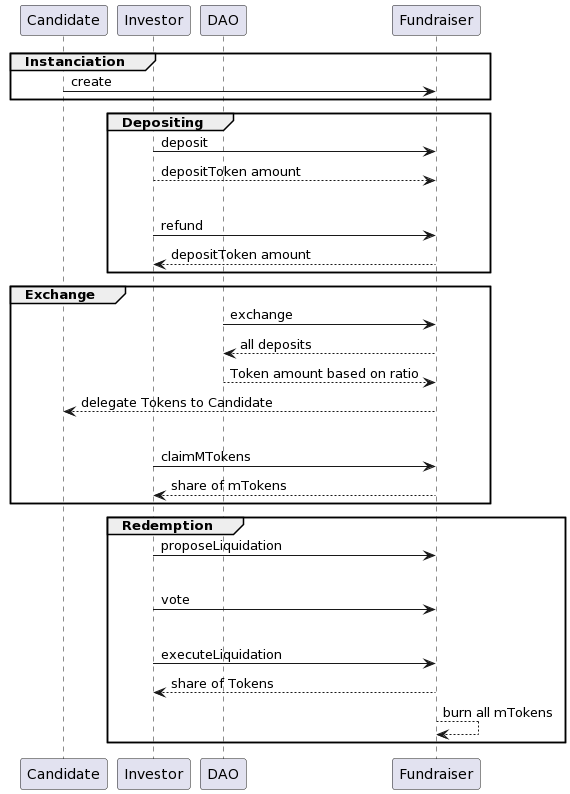
\includegraphics[width=\textwidth]{./img/molten-fundraiser-v1-seq-diag.png}
\caption{Sequence diagram}
\end{figure}

\end{document}
